\documentclass[12pt,fleqn]{article}\usepackage{../../common}
\begin{document}
Materyel Mekaniği - 11


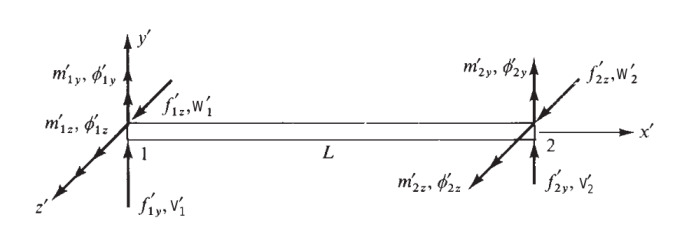
\includegraphics[width=20em]{phy_020_strs_11_01.jpg}


$x-z$ Duzlemi

$$
\frac{EI_y}{L^4}
\left[\begin{array}{cccc}
12L & -6L  & -12L & -6L^2 \\
    & 4L^3 & 6L^2 & 2L^3  \\
    &      & 12L  & 6L^2  \\
                  & 4L^3
\end{array}\right]
$$









\begin{minted}[fontsize=\footnotesize]{python}
from sympy import symbols, pprint, latex
from sympy.matrices import Matrix
import pandas as pd
pd.set_option('display.max_columns', None)

all_vars = ['u1','v1','w1','phi1x','phi1y','phi1z',\
            'u2','v2','w2','phi2x','phi2y','phi2z']
A,G,J,E,L,Iy,Iz = symbols("A,G,J,E,L,Iy,Iz")
\end{minted}

\begin{minted}[fontsize=\footnotesize]{python}
# x-z
vars1 = ['w1','phi1y','w2','phi2y']
M1 = pd.DataFrame([[12*L, -6*L**2,-12*L,-6*L**2],
                  [-6*L**2,4*L**3,6*L**2,2*L**3],
                  [-12*L,6*L**2,12*L,6*L**2],
                  [-6*L**2,2*L**3,6*L**2,4*L**3]],index=vars1)
M1.columns = vars1
M1 = M1 * (E*Iy/L**4 )
# x-y
vars2 = ['v1','phi1z','v2','phi2z']
M2 = pd.DataFrame([[12*L, 6*L**2,-12*L,6*L**2],
                  [6*L**2,4*L**3,-6*L**2,2*L**3],
                  [-12*L,-6*L**2,12*L,-6*L**2],
                  [6*L**2,2*L**3,-6*L**2,4*L**3]],index=vars2)
M2.columns = vars2
M2 = M2 * (E*Iz/L**4 )
\end{minted}

\begin{minted}[fontsize=\footnotesize]{python}
vars3 = ['u1','u2']
M3 = pd.DataFrame([[1,-1],[-1,1]],index=vars3)
M3.columns = vars3
M3 = M3 * (A*E/L)
\end{minted}

\begin{minted}[fontsize=\footnotesize]{python}
vars4 = ['phi1x','phi2x']
M4 = pd.DataFrame([[1,-1],[-1,1]],index=vars3)
M4.columns = vars4
M4 = M4 * (G*J/L)
\end{minted}

\begin{minted}[fontsize=\footnotesize]{python}
import sys; sys.path.append('../phy_020_strs_08')
import dfutil

M1f = dfutil.expand_dataframe(M1,all_vars)
M2f = dfutil.expand_dataframe(M2,all_vars)

M3f = dfutil.expand_dataframe(M3,all_vars)
M4f = dfutil.expand_dataframe(M4,all_vars)
Mall = M1f + M2f + M3f + M4f
#print (Mall.to_latex())
print (Mall)
\end{minted}

\begin{verbatim}
           u1             v1             w1   phi1x         phi1y  \
u1      A*E/L              0              0       0             0   
v1          0   12*E*Iz/L**3              0       0             0   
w1          0              0   12*E*Iy/L**3       0  -6*E*Iy/L**2   
phi1x       0              0              0   G*J/L             0   
phi1y       0              0   -6*E*Iy/L**2       0      4*E*Iy/L   
phi1z       0    6*E*Iz/L**2              0       0             0   
u2     -A*E/L              0              0       0             0   
v2          0  -12*E*Iz/L**3              0       0             0   
w2          0              0  -12*E*Iy/L**3       0   6*E*Iy/L**2   
phi2x       0              0              0  -G*J/L             0   
phi2y       0              0   -6*E*Iy/L**2       0      2*E*Iy/L   
phi2z       0    6*E*Iz/L**2              0       0             0   

              phi1z      u2             v2             w2   phi2x  \
u1                0  -A*E/L              0              0       0   
v1      6*E*Iz/L**2       0  -12*E*Iz/L**3              0       0   
w1                0       0              0  -12*E*Iy/L**3       0   
phi1x             0       0              0              0  -G*J/L   
phi1y             0       0              0    6*E*Iy/L**2       0   
phi1z      4*E*Iz/L       0   -6*E*Iz/L**2              0       0   
u2                0   A*E/L              0              0       0   
v2     -6*E*Iz/L**2       0   12*E*Iz/L**3              0       0   
w2                0       0              0   12*E*Iy/L**3       0   
phi2x             0       0              0              0   G*J/L   
phi2y             0       0              0    6*E*Iy/L**2       0   
phi2z      2*E*Iz/L       0   -6*E*Iz/L**2              0       0   

              phi2y         phi2z  
u1                0             0  
v1                0   6*E*Iz/L**2  
w1     -6*E*Iy/L**2             0  
phi1x             0             0  
phi1y      2*E*Iy/L             0  
phi1z             0      2*E*Iz/L  
u2                0             0  
v2                0  -6*E*Iz/L**2  
w2      6*E*Iy/L**2             0  
phi2x             0             0  
phi2y      4*E*Iy/L             0  
phi2z             0      4*E*Iz/L  
\end{verbatim}


[devam edecek]

Kaynaklar

[1] Bayramlı, {\em Fizik, Materyel Mekanigi 7}

\end{document}
